\documentclass{article}
\usepackage[utf8]{inputenc}

\title{Trabalho Prático 2 \\ Software Básico
\\ Ligador Simples}
\author{João Paulo Martino Bregunci - jpbregunci@gmail.com
\\ Ronald Davi Rodrigues Pereira - ronald.drp11@gmail.com}
\date{Novembro de 2016}

\usepackage{natbib}
\usepackage{graphicx}
\usepackage{indentfirst}

\begin{document}

\maketitle


\section{Introdução}
A tradução de código \textit{Assembly} para código de máquina é um dos problemas mais antigos da Ciência da Computação, dada a óbvia dificuldade da programação diretamente em código de máquina. Desse problema, iniciou-se a proposta desse trabalho que será a construção de um \textit{Ligador} simples, o qual é capaz de gerar código executável para a máquina \textit{Wombat2}. Este dado \textit{Ligador} em questão criado irá possibilitar a execução de funções presentes em diversos outros arquivos, retornando posteriormente ao \textit{Program Counter} a próxima instrução depois que a função foi chamada.

O \textit{Ligador} ao final de todo o processo é capaz de gerar um único arquivo executável, o qual contém todas as funções existentes, sendo o endereço de chamada de todas esses funções recalculado para ajustar-se a chamada de qualquer outra função presente no arquivo executável final.


\begin{figure}[!h]
\centering
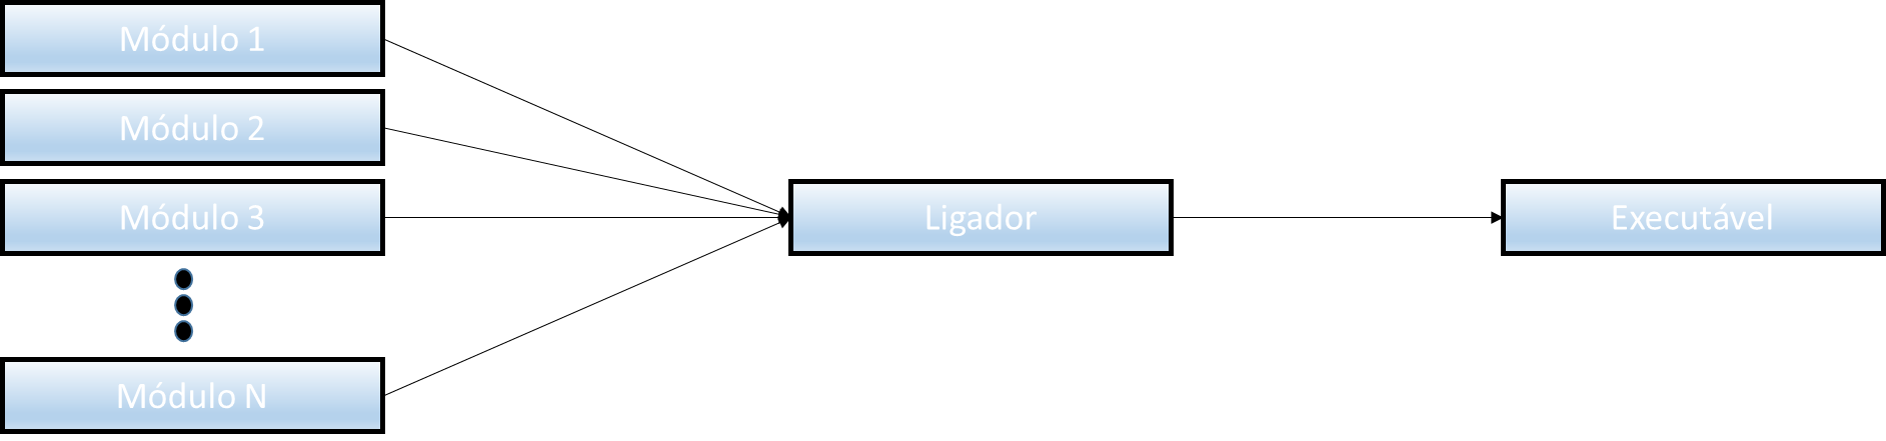
\includegraphics[scale=0.4]{ImagemTP2.png}
\caption{Diagrama que sintetiza o que o \textit{Ligador} faz}
\label{fig:trieExample}
\end{figure}

\section{Explanação do Problema}
\subsection{Apresentação do Problema}
Como enunciado anteriormente na Introdução, o problema consiste na implementação de \textit{Ligador} simples. Nesse contexto, notabiliza-se o maior problema o remanejamento do endereço das funções, ou seja, o recálculo do endereço de memória no qual a função se encontra depois que unem-se vários módulos ao executável principal.

\subsection{Decisões para Implementação}
Para a construção do ligador deve-se pontuar, primariamente, algumas condições simples para que o programa seja capaz de gerar um executável final sem que exista qualquer tipo de comportamento inesperado. Tais condições enunciadas são:

\begin{enumerate}
  \item Não deve haver nenhum espaço (ou tabulação) antes de uma linha que contém somente comentários, ou seja, em linhas que contém exclusivamente comentários o primeiro carácter deve ser exclusivamente o ponto e vírgula.
  \item Não devem haver nenhuma linha escrita no fim do programa (após os .datas), mesmo que sejam comentários, a fim de evitar comportamentos irregulares durante a execução.
  \item Não devem haver nenhum rótulo (label) no meio do programa Assembly que não esteja declarado em outro local do código, a fim de evitar o evidente problema de referências para procedimentos inexistentes.
  \item Labels devem começar com um \textit{underline}, tanto para jumps ou calls, a fim de padronizar de uma maneira simples a chamada de procedimentos.
  \item Labels referenciados pela pseudoinstrução .extern não devem conter um \textit{underline}, de forma a evitar problemas com a decodificação e comparação das demais ligações.
\end{enumerate}

Dito tal, o \textit{Ligador} é implementado primariamente por meio da criação de um novo arquivo, o qual é elaborado a partir de vários acessos a um \textit{array} com ponteiros para os arquivos dos módulos utilizados. A execução do \textit{assembler} remete fortemente ao trabalho prático anterior, só que agora há uma execução iterativa para cada módulo incluído.

Na implementação realizada o \textit{Program Counter} da \textit{main} tem início no valor zero e os módulos seguem logo abaixo continuando-se a contagem do \textit{PC}. Nessa implementação, uma ressalva muito importante que deve ser feita é que todos os \textit{.data} são impressos ao final de toda a execução da tradução. Esse procedimento só pode ser feito quando todos os \textit{.data} são salvos em uma lista encadeada, a qual ao final da primeira passada, grava os respectivos \textit{Program Counter} de todos esses \textit{.data}.

O procedimento acima pode ser um pouco de difícil compreensão ao leitor,contudo o esquema abaixo auxília a compreender entender a configuração final do arquivo.

\noindent==========================================

\noindent\textit{0 : começo da main\\
1::30 codigo da main\\
31 : finalização do main\\
32 : começo do módulo 1\\
33::48 código do módulo 1\\
49 : finalização do módulo 1\\
50 : inicio do .data da main\\
51 : finalização do .data da main\\
52 : início do .data do módulo 1\\
53 : finalização do .data do módulo 1\\
END\\
==========================================}

Caso seja do interesse do leitor utilizar o \textit{Ligador}, é necessário ir a pasta \textit{linker} e executar primeiramente o comando \textit{make all}. Após isso é possível utilizar o programa executando o comando:

\begin{center} \textit{/linker.exe output.mif main.a modulo1.a modulo2.a [...] modulon.a} \end{center}

\subsection{Detalhes de Implementação do Extern}

Cada \textit{label} e cada \textit{.data} é atribuído um ID do arquivo de entrada que ele se encontra, o que faz acessos a esses procedimentos somente serem possíveis localmente. Isso é realizado por motivos de segurança e modularização do código, a fim de evitar acessos inesperados a tais referências.

Os \textit{.externs} possuem uma mecânica de funcionamento de maneira similar aos \textit{labels} e aos \textit{.datas}. Na primeira passada são salvos na lista \textit{"ext"} o endereço da memória de instruções e o endereço destino do \textit{label} no seu respectivo módulo. Esse procedimento é útil, pois em cada chamada \textit{.extern}, basta substituir a pseudoinstrução por uma instrução \textit{call}, apontando para o endereço salvo na lista \textit{"ext"}. Portanto, todos os \textit{.extern} ao final da execução são traduzidos para uma instrução \textit{call}, já que endereço de destino já foi previamente calculado para o novo arquivo.


\section{Casos de Teste}

Abaixo consta a imagem de todos os casos de teste para as diversas operações descritas nas especificações do trabalho. As imagens todas são referentes a simulações feitas na máquina \textit{Wombat2}.

\begin{figure}[!]
\centering
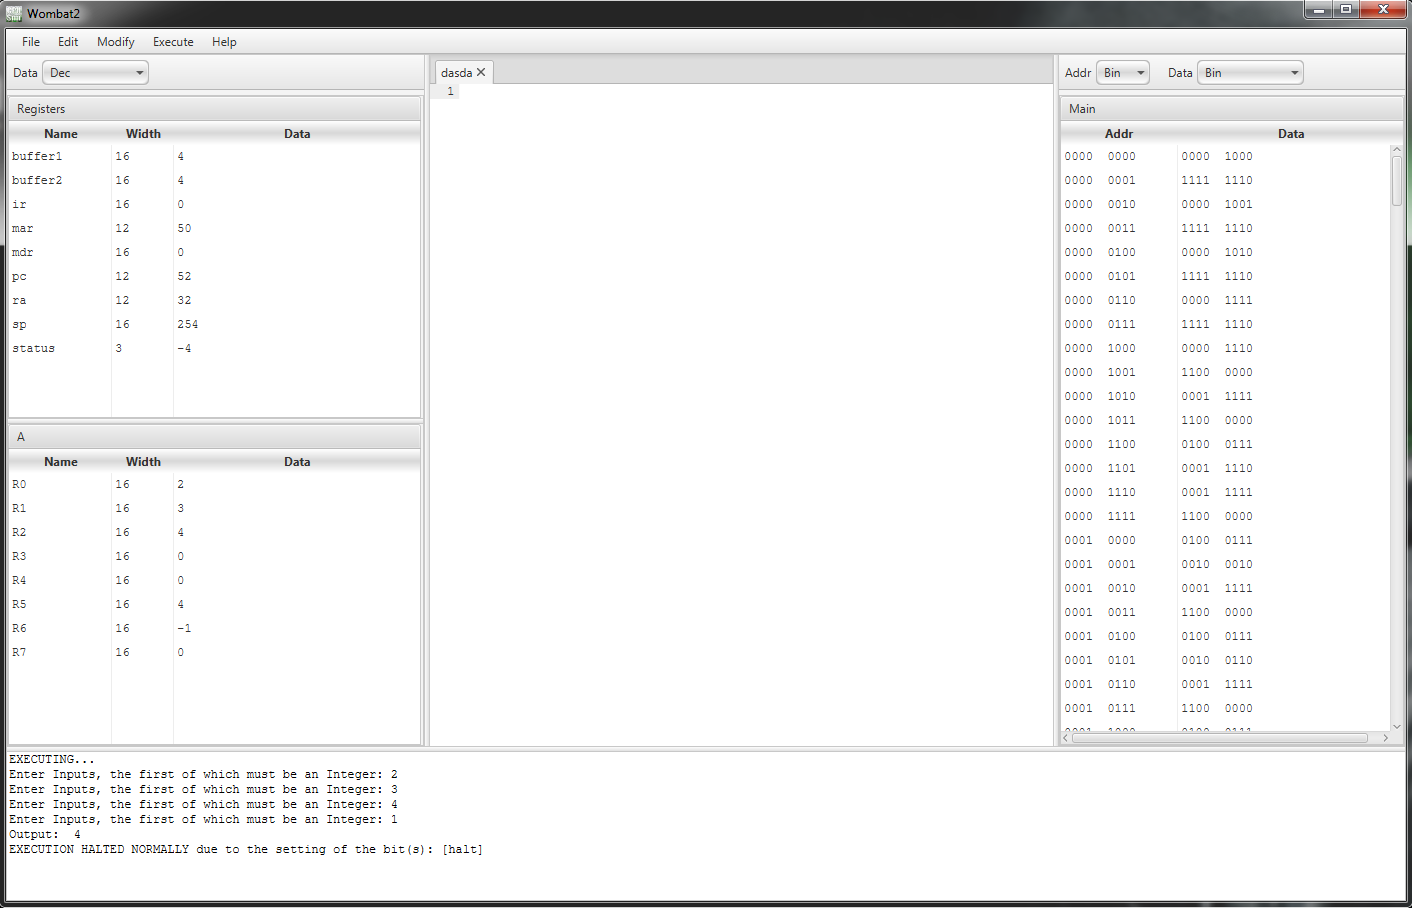
\includegraphics[scale=0.34]{1.png}
\caption{Imagem do programa para a operação 1 (exibir o maior entre os números)}
\label{fig:ibagem1}
\end{figure}

\begin{figure}[!]
\centering
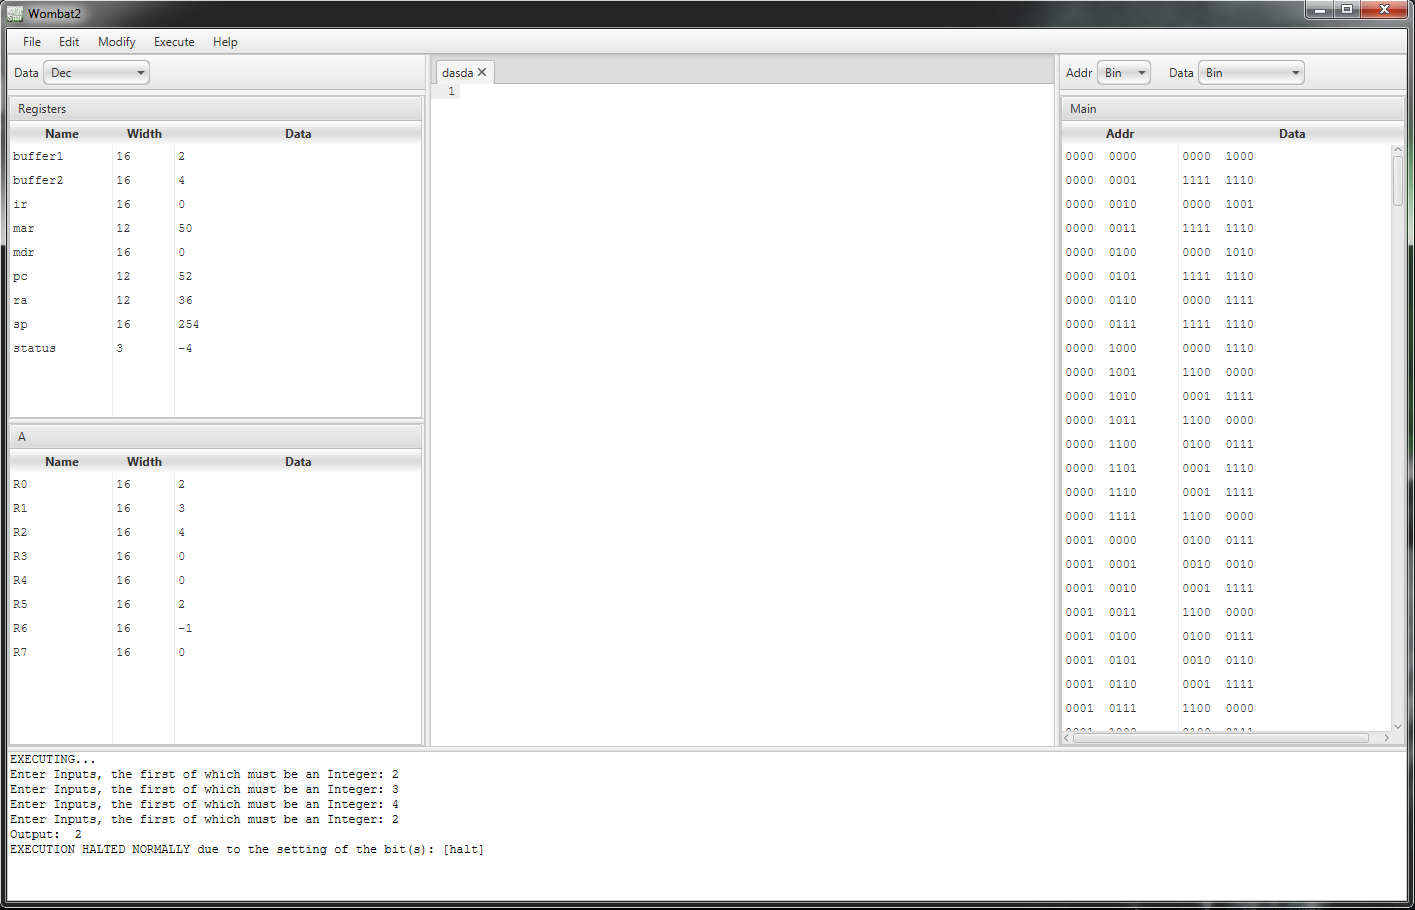
\includegraphics[scale=0.34]{2.png}
\caption{Imagem do programa para a operação 2 (exibir o menor entre os números)}
\label{fig:ibagem2}
\end{figure}

\begin{figure}[!]
\centering
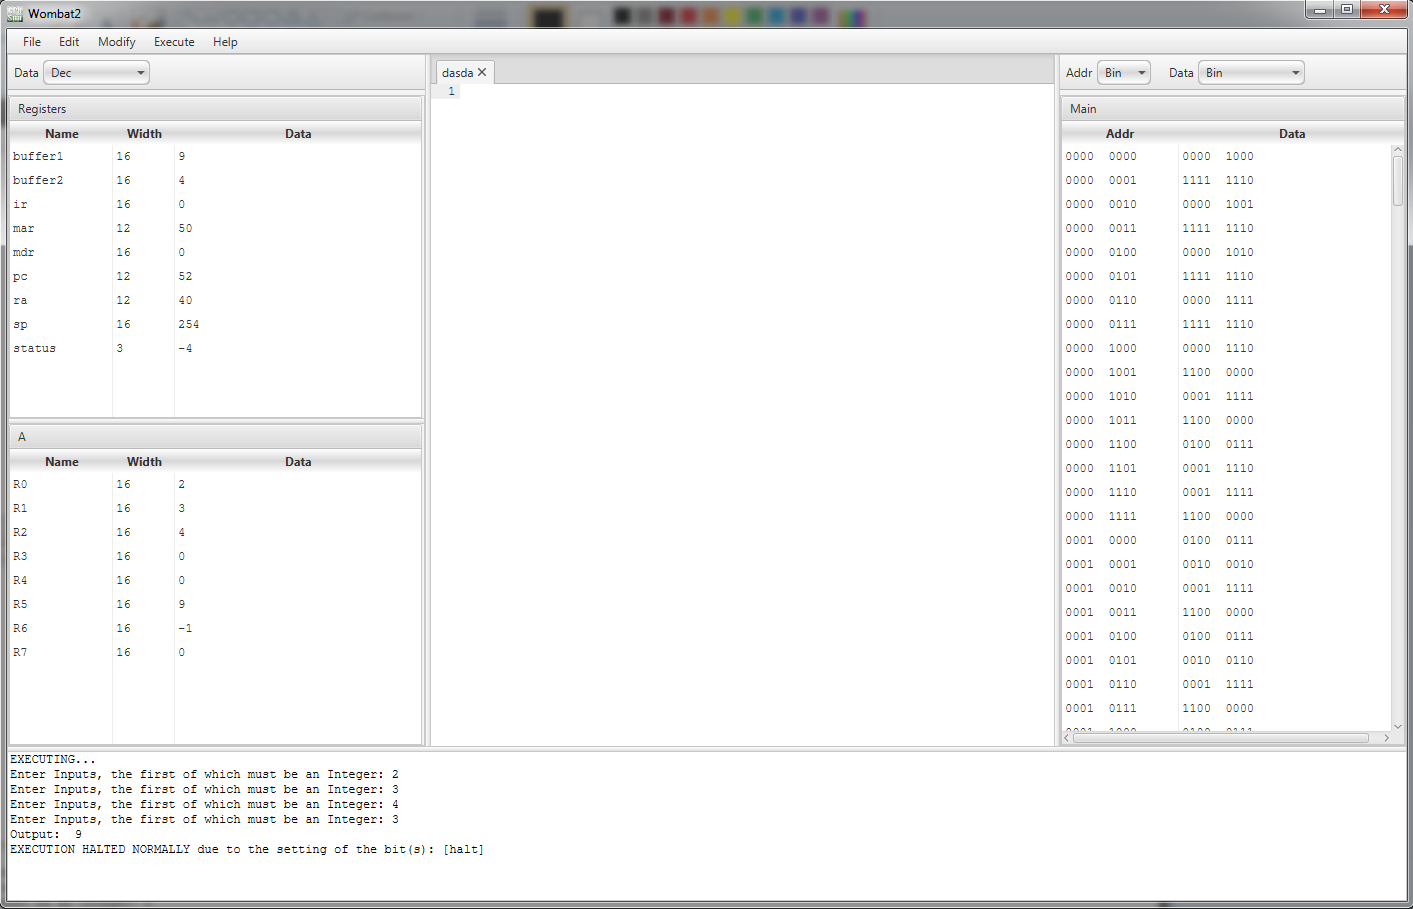
\includegraphics[scale=0.34]{3.png}
\caption{Imagem do programa para a operação 3 (exibir a soma entre os números)}
\label{fig:ibagem3}
\end{figure}


\begin{figure}[!]
\centering
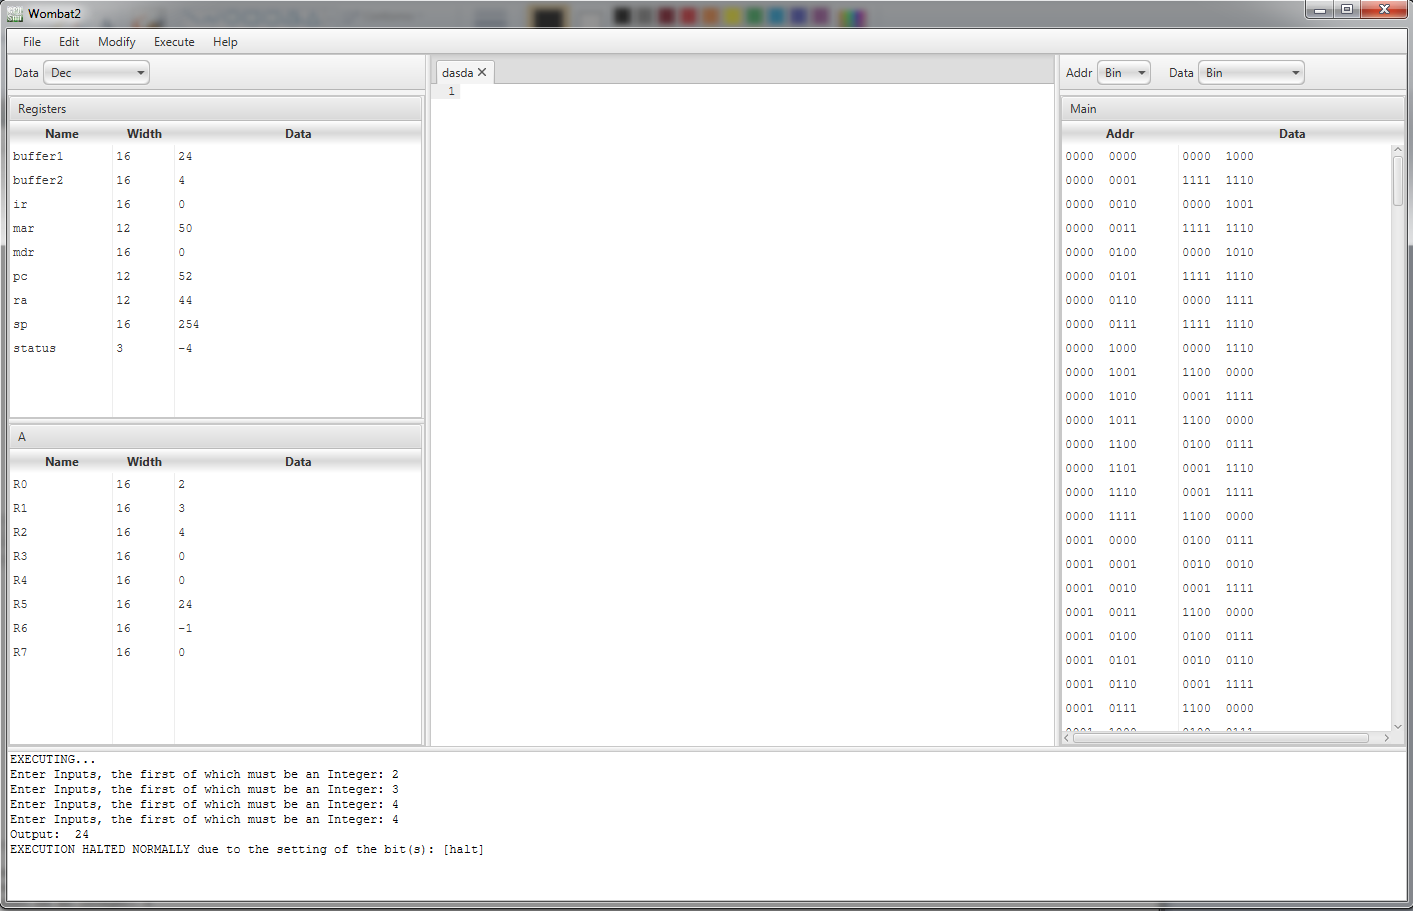
\includegraphics[scale=0.34]{4.png}
\caption{Imagem do programa para a operação 4 (exibir a multiplicação entre o números)}
\label{fig:ibagem4}
\end{figure}

\begin{figure}[!]
\centering
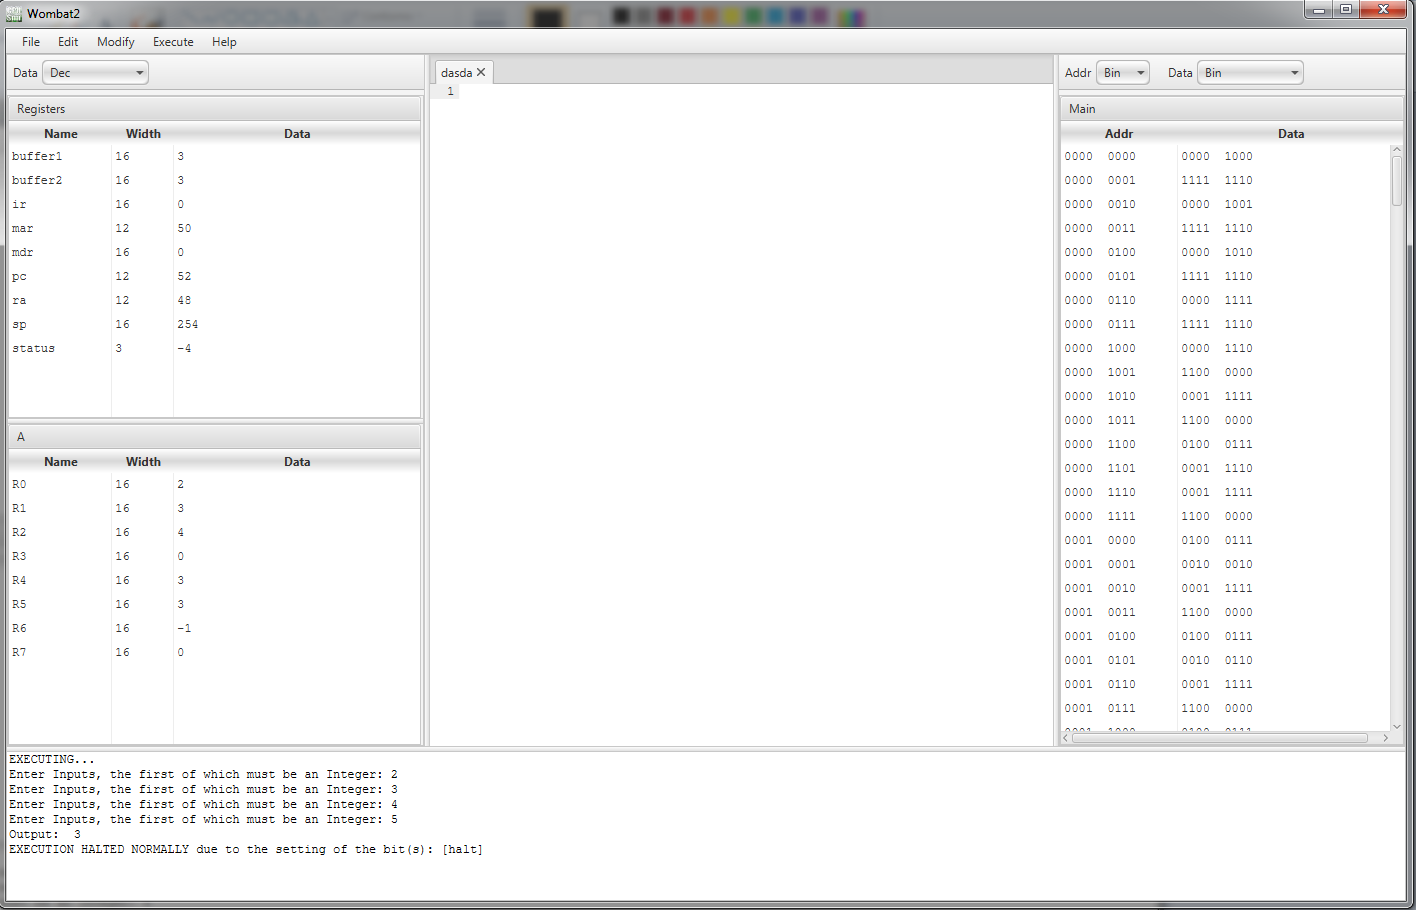
\includegraphics[scale=0.34]{5.png}
\caption{Imagem do programa para a operação 5 (exibir a média aritmética entre os números)}
\label{fig:ibagem5}
\end{figure}


\goodbreak\newpage\section{Conclusão}

Por meio desse trabalho foi possível expandir ainda mais o conhecimento sobre a geração de código máquina, a partir de um código \textit{Assembly}. Foi gerado ao final desse trabalho, um \textit{Ligador} completamente funcional capaz de gerar eficientemente um código executável para a máquina \textit{Wombat2}, utilizando para isso, diversos procedimentos de vários módulos simultaneamente.


\begin{thebibliography}{9}

\bibitem{knuthwebsite}
Colby College, Official CPUsim Website
\\\texttt{http://www.cs.colby.edu/djskrien/CPUSim/}
\end{thebibliography}
\end{document}
